%% ============================================================
%%  CHAPTER 5 — Proposed Solution: FAIR-FRFT Architecture
%%  Ethics in AI: Emphasis on Fairness
%%  CSC-391 Technical Communication, IIT Roorkee
%% ============================================================
 
\chapter{Targeting a Critical Gap in Deepfake Detectors}
\label{ch:proposed}
 
\vspace{0.5em}
\noindent\rule{\textwidth}{0.4pt}
\textbf{Declaration of Contributions:} This chapter was developed by
\textit{Siddharth Gupta} and \textit{Aryan Choudhary}, the former contributed to the conceptualisation and theoretical design of the autoencoder architecture and the debiasing framework, based on an extensive review of existing literature, while the later contributed to the theoretical formulation and design of the CVaR-based fairness module.
\noindent\rule{\textwidth}{0.4pt}
\vspace{1em}

\bigskip


 
This chapter presents \textbf{FAIR-FRFT} (\emph{Fairness-Aware
Fractional Fourier Transform for Deepfake Detection}), our proposed
framework for demographically fair deepfake detection.  Unlike prior
methods that append fairness as a post-hoc constraint on top of an
existing architecture, FAIR-FRFT treats fairness as a
\emph{fundamental design principle}, embedding demographic invariance
directly into the representation-learning process through three
tightly coupled components: (i) a hybrid spatial--frequency encoder
driven by the Fractional Fourier Transform, (ii) an adversarial
autoencoder with a Gradient Reversal Layer, and (iii) a
CVaR-based tail-risk fairness objective.  Together, these components
ensure that the learned latent representations are simultaneously
deepfake-discriminative and demographic-agnostic.

% ------------------------------------------------------------------
\section{Problem Statement}
\label{sec:problem_statement}
% ------------------------------------------------------------------

Deepfake detectors are not necessarily fair across demographic groups.
A model may achieve strong overall accuracy while still producing
systematically different error rates for different communities. This occurs when the detector learns correlations present in the training data that do not generalise fairly across groups.

In the context of deepfake detection, such bias is especially problematic because the impact of an error can be severe. A detector that performs well on one community but poorly on another may create uneven trust and unequal risk. 

\subsubsection{Illustrative Scenario}
\label{subsec:problem_example}

Consider an election setting in which a deepfake speech is circulated
publicly against a political candidate. Suppose the detector, due to its inherent bias and limitations in learned representations, incorrectly labels the speech as genuine rather than synthetic. Such a failure may allow the manipulated content to spread widely, potentially triggering public unrest, misleading voters and damaging the candidate's reputation. This example highlights why fairness in deepfake detection is not merely a technical concern, but a \emph{matter of real-world safety and social responsibility}.
 
% ------------------------------------------------------------------
\section{Overview of the FAIR-FRFT Architecture}
\label{sec:architecture_overview}
% ------------------------------------------------------------------
 
Figure~\ref{fig:fairfrft_architecture} provides a complete view of the
FAIR-FRFT pipeline.  At the highest level, the framework comprises
four functional blocks:
 
\begin{enumerate}
  \item \textbf{FrFT pre-processor}  The input image $\mathbf{x}$
        is mapped to the hybrid spatial frequency domain via the
        Fractional Fourier Transform, yielding frequency maps
        $\mathbf{x}' = \mathcal{F}_\alpha^{(d)}(\mathbf{x})$.
  \item \textbf{Adversarial autoencoder}  An encoder
        $E_\theta$ compresses $\mathbf{x}'$ into a latent
        representation $\mathbf{z}$; a decoder $G_\theta$
        reconstructs the spatial-domain image $\hat{\mathbf{x}}$
        from $\mathbf{z}$.  The cycle is closed by re-encoding the
        reconstruction for latent consistency.
  \item \textbf{Demographic adversary}  A demographic classifier
        $D_\phi$ attempts to predict the protected group $g$ from
        $\mathbf{z}$.  Gradient reversal forces the encoder to
        \emph{maximise} the adversary's error, thereby stripping
        demographic information from the latent space.
  \item \textbf{Binary Real/Fake classifier}  After the encoder has
        converged to a fair representation, a lightweight
        classifier $C_\psi$ is trained on the frozen $\mathbf{z}$
        to detect real versus fake faces.
\end{enumerate}
 
% ------------------------------------------------------------------
\section{Fractional Fourier Transform Pre-processing}
\label{sec:frft_preproc}
% ------------------------------------------------------------------
 
The Fractional Fourier Transform (FrFT), introduced in
Section~\ref{sec:frft}, serves as the input representation for
FAIR-FRFT.  For an order parameter $\alpha \in [0,1]$, the
2-D FrFT of an image $\mathbf{x}$ is computed channel-wise as:
\begin{equation}
  \mathbf{x}' = \mathcal{F}_\alpha^{(d)}(\mathbf{x})
  \label{eq:frft_preproc}
\end{equation}

\begin{equation}
  \mathcal{F}_\alpha[f](u)
  = e^{-i\pi u^2 \cot\alpha}
    \cdot \mathrm{FFT}\!\left[f(t)\,e^{-i\pi t^2 \cot\alpha}\right]\!(u\csc\alpha)
\end{equation}

\begin{figure}[h]
    \centering
    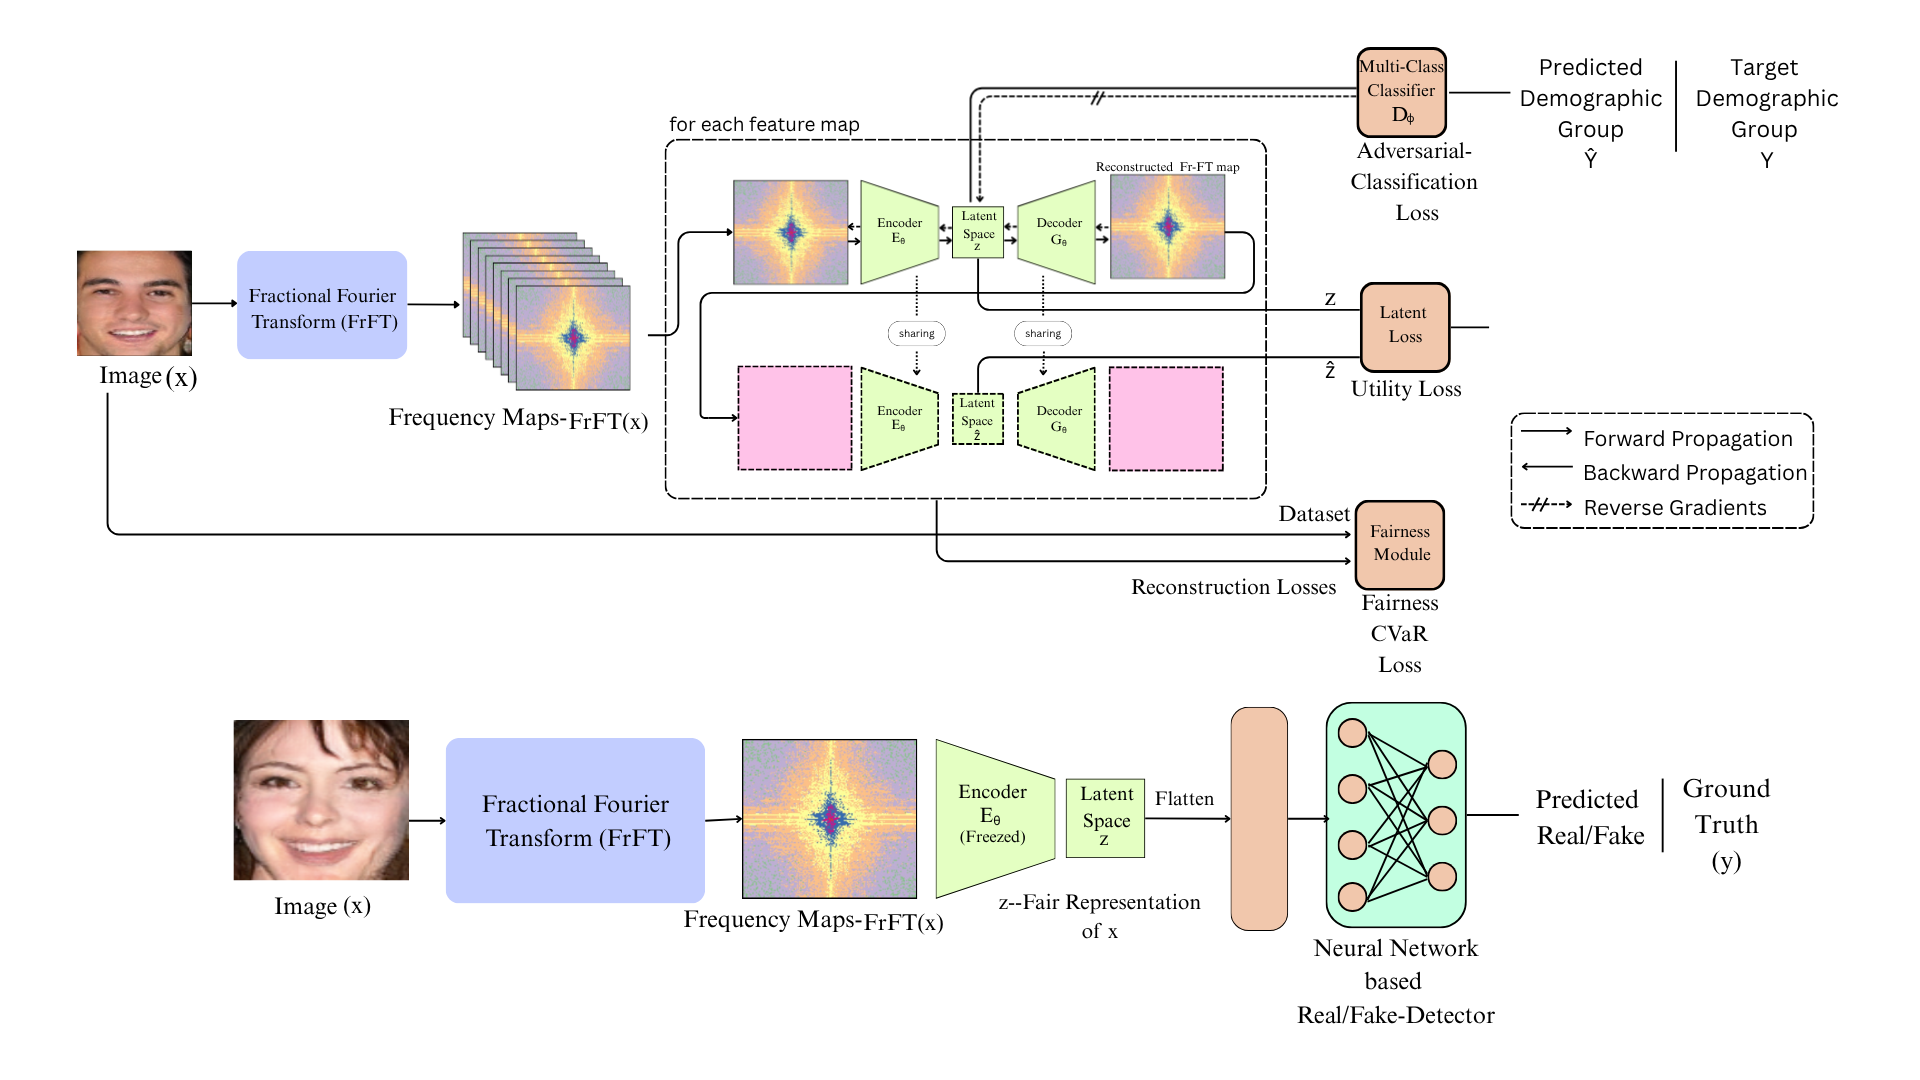
\includegraphics[width=1\textwidth]{images/FAIRFRFT.png}
    \caption{FAIR-FRFT Architecture. Top: FrFT-transformed input $x'$ is encoded by $E_{\theta}$ into latent $z$, reconstructed by $G_{\theta}$ to $\hat{x}$, and re-encoded for consistency. The model includes demographic adversary $D_{\phi}$, real/fake head $R_{\psi}$, and CVaR fairness loss. Bottom: After training, the encoder is frozen and a classifier predicts real/fake labels from the learned fair representation.}
    \label{fig:fairfrft_architecture}
\end{figure}

 
% ------------------------------------------------------------------
\section{Adversarial Autoencoder}
\label{sec:adv_ae}
% ------------------------------------------------------------------
 
\subsubsection{Encoder and Decoder}
\label{subsec:enc_dec}
 
The encoder $E_\theta : \mathbb{R}^{H \times W \times C}
\to \mathbb{R}^d$ maps the FrFT-transformed image to a
$d$-dimensional latent vector:
\begin{equation}
  \mathbf{z} = E_\theta(\mathbf{x}').
  \label{eq:encoder}
\end{equation}
We implement $E_\theta$ as a three-layer CNN with filter counts 32, 64 and 128. Layer Normalization after each convolution and additive Gaussian noise ($\sigma = 0.05$) for regularisation. Critically, no non-linear activation function is applied after the final layer; this preserves the sign of latent activations, which carries phase information propagated from the FrFT.
 
The decoder $G_\theta : \mathbb{R}^d \to
\mathbb{R}^{H \times W \times C}$ reconstructs the spatial-domain
image:
\begin{equation}
  \hat{\mathbf{x}} = G_\theta(\mathbf{z}).
  \label{eq:decoder}
\end{equation}
$G_\theta$ is a symmetric CNN with transposed convolutions and skip connections from the corresponding encoder layers, mirroring the U-Net paradigm to recover fine spatial detail. The reconstructed image is then re-processed through FrFT and re-encoded:
\begin{equation}
  \hat{\mathbf{x}}' = \mathcal{F}_\alpha^{(d)}(\hat{\mathbf{x}}),
  \qquad
  \hat{\mathbf{z}} = E_\theta(\hat{\mathbf{x}}')
  \label{eq:cycle}
\end{equation}
 
\subsubsection{Latent Consistency Objective}
\label{subsec:lat_consistency}
 
Rather than enforcing pixel-level reconstruction which would force the model to attend to demographic appearance details we enforce \emph{latent-space consistency}. The latent consistency loss comprises an $\ell_2$ term and a cosine-similarity term:
\begin{equation}
  \mathcal{L}_{\mathrm{lat}}
  \;=\;
  \bigl\|\hat{\mathbf{z}} - \mathrm{sg}(\mathbf{z})\bigr\|_2^2
  \;+\;
  \beta\,\bigl(1 - \cos(\hat{\mathbf{z}},\,\mathrm{sg}(\mathbf{z}))\bigr),
  \quad \beta = 1.0
  \label{eq:lat_loss}
\end{equation}
where $\mathrm{sg}(\cdot)$ denotes the \emph{stop-gradient} operator (the target $\mathbf{z}$ is treated as a constant during the backward pass). By constraining the encoder to produce latents that survive a decode re-encode cycle, we encourage the representation to capture \emph{semantic deepfake cues} (which persist through reconstruction) while discarding superficial appearance variations such as skin tone and facial structure (which are smoothed away by the decoder).
 
% ------------------------------------------------------------------
\section{Adversarial Demographic Debiasing via Gradient Reversal}
\label{sec:adv_debias}
% ------------------------------------------------------------------
 
\subsubsection{Demographic Classifier}
\label{subsec:dem_clf}
 
A demographic classifier $D_\phi : \mathbb{R}^d \to \mathbb{R}^{|\mathcal{G}|}$ maps the latent representation to a probability distribution over demographic groups.  It is implemented as a two-layer MLP with Layer Normalisation and Max-Norm constraints ($c_{\max} = 3.0$) to bound its complexity.  The adversarial classification loss is:
\begin{equation}
  \mathcal{L}_{\mathrm{adv\text{-}clf}}
  \;=\;
  \mathbb{E}_{\mathbf{x},g}\!\bigl[
    \mathrm{CE}\!\bigl(D_\phi(\mathrm{GRL}(\mathbf{z})),\, g\bigr)
  \bigr],
  \label{eq:adv_clf}
\end{equation}
where $\mathrm{GRL}(\cdot)$ is the Gradient Reversal Layer defined in Eq.~\ref{eq:grl}.
 
\subsubsection{Minimax Training Objective}
\label{subsec:minimax}
 
The encoder and demographic classifier engage in a minimax game:
\begin{equation}
  \min_{\theta}\;\max_{\phi}\;
  \mathcal{L}_{\mathrm{AE}}
  \;=\;
  \lambda_{\mathrm{lat}}\,\mathcal{L}_{\mathrm{lat}}(\theta)
  \;+\;
  \lambda_{\mathrm{fair}}\,\mathcal{L}_{\mathrm{fair}}(\theta)
  \;-\;
  \lambda_{\mathrm{adv}}\,\mathcal{L}_{\mathrm{adv\text{-}clf}}(\theta,\phi).
  \label{eq:minimax}
\end{equation}
The negative sign on $\mathcal{L}_{\mathrm{adv\text{-}clf}}$ causes the encoder to \emph{maximise} the adversary's classification error equivalently, to remove demographic information from $\mathbf{z}$.  The GRL makes this implicit: during the forward pass it acts as the identity; during back-propagation it negates the gradient by the reversal strength $\lambda_{\mathrm{grl}}$ (Eq.~\ref{eq:grl}),  avoiding the need for alternating optimisation.

 
% ------------------------------------------------------------------
\section{CVaR Fairness Loss}
\label{sec:cvar_fair}
% ------------------------------------------------------------------
 
Adversarial debiasing removes demographic information from $\mathbf{z}$ in an \emph{average} sense, but may still leave vulnerable subgroups under-served.  To protect these subgroups, we propose to augment the training objective with a \emph{group-level CVaR} fairness loss (see Section~\ref{sec:cvar}):
\begin{equation}
  \mathcal{L}_{\mathrm{fair}}
  \;=\;
  \max_{y,\,a}\;
  \mathrm{CVaR}_\alpha\!\bigl(\ell(\mathbf{x}, y) \mid y, a\bigr),
  \label{eq:fair_loss}
\end{equation}
where $y \in \{0,1\}$ is the real/fake label, $a$ is the demographic group, and the inner CVaR is taken over the loss distribution of that demographic--label cell.  Taking the $\max$ over all $(y, a)$ combinations focuses optimisation on the \emph{worst-performing subgroup}, ensuring Equalized Odds across the population.  This connects directly to the group-level CVaR formulation of Eq.~\ref{eq:group_cvar}.
 
% ------------------------------------------------------------------
\section{Model Pipeline}
\label{sec:training_strategy}
% ------------------------------------------------------------------
 
The proposed model pipeline ought to be trained in two stages:
 
\subsubsection{Stage 1 : Fair Representation Learning}
\label{subsec:stage1}
The adversarial autoencoder is to be trained end-to-end to learn demographic-agnostic semantically meaningful representations:
\begin{equation}
  \theta^{(1)},\,\phi^*
  \;=\;
  \operatorname*{arg\,min}_{\theta}\;
  \operatorname*{arg\,max}_{\phi}\;
  \mathcal{L}_{\mathrm{AE}}(\theta, \phi).
  \label{eq:stage1}
\end{equation}

\subsubsection{Stage 2 : Binary Classification}
\label{subsec:stage2}
 
Once the encoder has converged, $E_\theta$ is \emph{frozen} and a separate real/fake classifier $C_\psi$ ought to be trained on the fixed representations:
\begin{equation}
  \psi^*
  \;=\;
  \operatorname*{arg\,min}_{\psi}\;
  \mathcal{L}_{\mathrm{clf}}(\psi;\,\theta^{(1)})
  \;=\;
  \mathbb{E}_{\mathbf{x},y}\!\bigl[
    \mathrm{CE}\!\bigl(C_\psi(\mathbf{z}),\,y\bigr)
  \bigr].
  \label{eq:stage2}
\end{equation}
Decoupling representation learning from classification prevents the
classifier's cross-entropy gradient from re-introducing demographic
bias into $\mathbf{z}$.
 
 
% ------------------------------------------------------------------
\section{Chapter Summary}
\label{sec:ch5_summary}
% ------------------------------------------------------------------
 
This chapter presented FAIR-FRFT, our proposed fairness-aware
deepfake detection framework.  The key design decisions and their
justifications are:
 
\begin{itemize}
  \item \textbf{FrFT pre-processing} maps images into a hybrid spatial frequency domain where deepfake artefacts are more discriminative and less entangled with demographic
        appearance features.
  \item \textbf{Latent consistency training} replaces pixel reconstruction with a semantic cycle-consistency objective, preventing the autoencoder from memorising demographic appearance cues.
  \item \textbf{Gradient Reversal} implements adversarial debiasing within a single forward--backward pass, actively removing demographic information from the latent space without alternating optimisation. 
  \item \textbf{CVaR fairness loss} complements adversarial 
        debiasing by directly penalising worst-case subgroup  performance, linking the training objective to the Equalized Odds fairness criterion.
  \item \textbf{Two-stage training} decouples fair
        representation learning from task-specific
        classification, preventing the classifier's gradient
        from re-introducing bias.
\end{itemize}